\subsection{Backend Arkitektur}

I dette afsnit redegøres for arkitekturen af backend containeren. Dokumentet vil først komme med en kort redegørelse for MVC mønstrets opbygning og dets bidrag til arkitekturen. Dernæst gennemgås de relevante krav hvad angår backenden, disse krav bruges som input til arkitekturen. Med kravene på plads præsenteres et C3 diagram over backend’en, som viser hvordan Web api’et opbygges. Til slut præsenteres REST principper samt hvordan de anvendes.
Systemets backend vil bestå af et Web API udviklet i frameworket ASP.NET Core. Web API’et skal give mulighed for containerne Frontend og GameEngine at tilgå databasen igennem HTTP request/responses, for at hente og sende den nødvendige data til databasen. Hertil skal backend’en sørger for Authentication og Authorization af de indkommende kald.\\

\subsubsection{MVC}
Selve Web API’ets arkitektur bygges op omkring MVC (Model-View-Controller) mønstret. En illustration af MVC mønstrets struktur kan ses på \autoref{fig:Arkitektur-Backend-MVC} (mangler ref til kilde).

\begin{figure}[H]
\centering
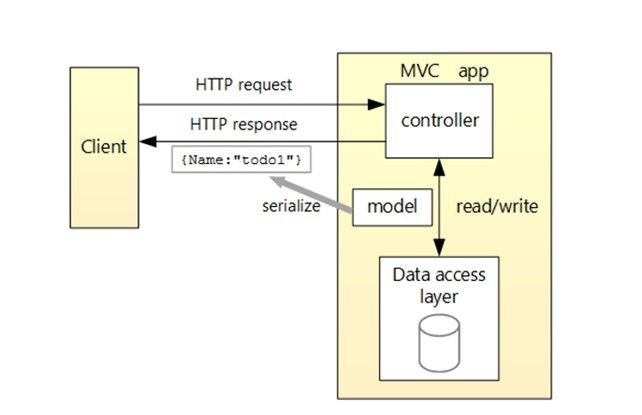
\includegraphics[width = \textwidth]{02-Body/Images/MVC_pattern.JPG}
\caption{Illustration af MVC pattern, bestående af clienter, controller, modeller, og et DAL. som viser hvordan de kommunikerer}
\label{fig:Arkitektur-Backend-MVC}
\end{figure}

Som det kan ses på figuren består mønstret overordnet af 4 dele; client, controller, model og et DAL (Data Access Layer). Da der er tale om et Web API gøres der ikke brug af view moduller. De enkelte moduler har følgende ansvar.

\textbf{Client:}\\
Clientens rolle er at kontakte Web API’et med henblik på at få udført en service, eksempel at logge ind.\\
\textbf{Controller:}\\
Controllernes ansvar er at håndterer indkommende kald fra clienten, og route til de rigtige Http endpoints, hvorefter databasen kontaktes igennem DAL.\\
\textbf{DAL:}\\
DAL’s ansvar er at kontakte og administere kommuikation med databasen i form af queries. Det er også her relationerne imellem data objekterne defineres.\\
\textbf{Model:}\\
Modelernes ansvar er at håndtere og definere den data som kan sendes frem og tilbage mellem clienten og databasen, de sørger altså for at binde alle modulerne sammen, således at der er enighed omkring hvordan data objekterne ser ud.
Som det kan ses passer MVC mønstret perfekt til den funktionalitet der ønskes. Mønstret gør det muligt at lave en logisk gruppering af relaterede opgaver, og er med til at sikre høj samhørighed i applikationen, ved at de enkelte ansvarsområder fordeles ud på hver sine moduler. På figur xxx \textbf{MANGLER REF} ses det tydeligt hvordan koblingen mellem de enkelte moduler holdes på et lavt niveau, hvilket gør det lettere at bygge videre på og tilføje ny funktionalitet.

\subsubsection{C3-Model for backend}

De relevante user stories for backend containeren udvælges. Disse omhandler håndtering af bruger konti, samt loading og saving af et game state.
 
\begin{itemize}
\item User Story 1 : Log in
\item User Story 2 : Opret Bruger
\item UserStory 7 : Exit Menu -\g Save and Exit
\item UserStory 17 : Main Menu -\g Load List Game
\item UserStory 18 : Main Menu -\g Load Game -\g Load
\item UserStory 19 : Main Menu -\g Load Game -\g Delete Game
\end{itemize}
Af de ikke funktionelle krav er følgende krav relevante:
\begin{itemize}
\item Skal kunne gemme maksimalt 5 save games
\item Skal kunne loade et spil indenfor maksimalt 5 s.
\item Skal kunne respondere indenfor maksimalt 5 s.
\end{itemize}
De ikke funktionelle krav tages hånd om under designet og implementeringen af backenden.
For ydderligere detaljer omkring funktionelle og ikke funktionelle krav henvises til Bilag x


Der bygges videre på C4 modellen for systemet , et level 3 component diagram over backend containeren udarbejdes, som viser hvilke componenter containeren indeholder, deres ansvarsområder, hvordan de kommunikere indbyrdes og med de omkring liggende containere, samt hvilke teknologier der anvendes i implementeringen, diagrammet kan ses på \autoref{fig:Arkitektur-Backend-C3}. 


\begin{figure}[H]
\centering
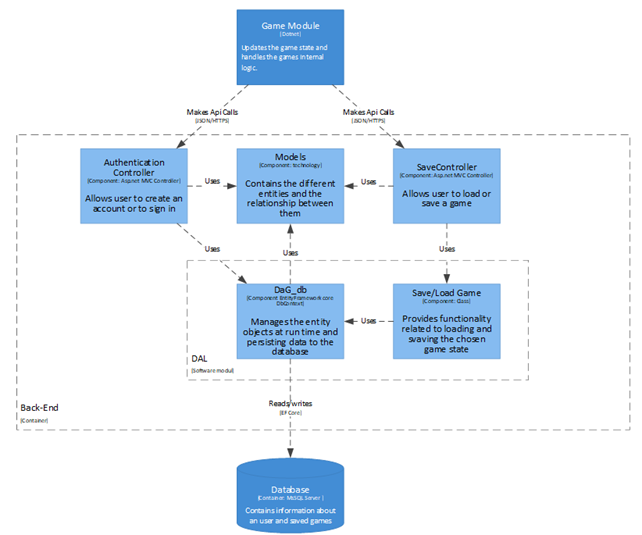
\includegraphics[width = \textwidth]{02-Body/Images/Backend_C3.PNG}
\caption{C3-Model over Backend container,figuren giver et overblik over de componenter backenden består, samt hvordan disse kommunikere indbyrdes og med omkring liggende containere.}
\label{fig:Arkitektur-Backend-C3}
\end{figure}

Figuren illustrerer en lagdelt struktur, hvor der ses en client som kalder ned i controllerne Authentication og Save Controller, som kalder videre til DAL, som så tilgår databasen denne kommunikationsvej går begge veje.

\textbf{Client:}\\
Der eksisterer en client, som kommunikerer med backenden Game Module. Game Module’s kald til backenden kan overordnet set indeles i to undergrupper, bruger håndtering og save håndtering. Bruger håndtering indeholder kald som omhandler login og registreing  (User story 1 og 2), hvor save håndtering omhandler loading og saving af Game state (User story 7, 17, 18 og 19). Kommuniaktionen her vil foregå ved netværkskald med protokolen HTTPS. Clienten udfører request/response kald til backenden igennem specifikke URL’s. For at data objekterne kan sendes frem og tilbage med HTTPS kald skal disse seralizeres og deseralizeres mellem JSON-objekter og .Net objekter.\\
\textbf{Controller:}\\
Inde i backenden anvendes ASP. Net MVC controllere(Mangler ref)   til at modtage og svare på kald fra clienten. Der laves en controller for Bruger håndtering og en controller for Save håndtering. Hver request mappes til en specifik controller. Controllerne vil så indeholde action metoder, som udføres når den modtagere et kald. Når controlleren har udført sin action retuneres et Action Result, hvor i et data objekt kan wrappes eller den kan indeholde en fejlmeddelse hvis noget går galt.\\
\textbf{DAL:}\\
De to controllere kalder som sagt videre ned i DAL laget, dette lag består af en database kontekst DaG\_db og en hjælper klasse til at udfører Queries. Her gøres brug af EF (Entity Framework) Core, som gør det muligt at arbejde med DbContext klassen, denne bruges til skabe en kontekst af databasen hvor i de enkelte modeller kan mappes til entities med Db<set>. Dette giver mulighed for at udfører operationer/queries på SQL databasen ved hjælp af LINQ (Language-Integrated Query).\\
\textbf{Model:}\\
Modellerne fungerer som bindeledet mellem alle komponenterne, de definere den data som der arbejdes på, og vil blot bestå af en række C\# klasser.\\

Som det kan ses passer MVC mønstret perfekt til den funktionalitet der ønskes. Mønstret gør det muligt at lave en logisk gruppering af relaterede opgaver, og er med til at sikre høj samhørighed i applikationen, ved at de enkelte ansvarsområder fordeles ud på hver sine moduler. På figur 1 \textbf{MANGLER REF HER} ses det tydeligt hvordan koblingen mellem de enkelte moduler holdes på et lavt niveau, hvilket gør det lettere at bygge videre på og tilføje ny funktionalitet.


\subsubsection{REST}
Web Api’et arkitektur vil gøre brug af REST principper, for ikke at gøre data overførelserne for komplekse og for at overholde SoC, ved at adskille repræsentationen og dataen fra hinanden, på den måde sikres det at dataen, kan blive repræsenteret på den ønskede måde, og ikke er tvunget til at blive gemt på en specifikt måde.
Dette kommer til udtryk ved følgende 5 REST principper(Mangler ref)  som søges opnået:
\begin{enumerate}
 \item Alle de data objekter der arbejdes med tilhører en bestemt unique URI. Dataen hentes, sendes og manipuleres igennem standard HTTP metoder som (GET, POST, PUT, DELETE).
 \item Der arbejdes ud fra en client/server arkitektur med data som resource. 
 \item Web Api’et er stateless, hvilket vil sige der gemmes ikke nogen tilstand omkring clienten på server siden.
 \item Der arbejdes ud fra en lagdelt struktur, som betyder at hver component kun kan se de componenter som grænser op til den selv.
 \item Der anvendes Cashing på server siden (Dette vil ikke blive implementeret).
\end{enumerate}

\subsubsection{Konlusion}

Systemets backend består at Web Api, som bygges op omkring MVC mønstret, som gør det muligt at lave en logsik gruppering af den enkelte funktionalitet. Web Api’et vil ligeledes gøre brug af REST principper for at adskille data resourcerne fra deres repræsentation på clientens side.

\newpage
